\documentclass{standalone}
\usepackage{tikz}
\usetikzlibrary{positioning,calc}
\usepackage{amsmath}  

\begin{document}
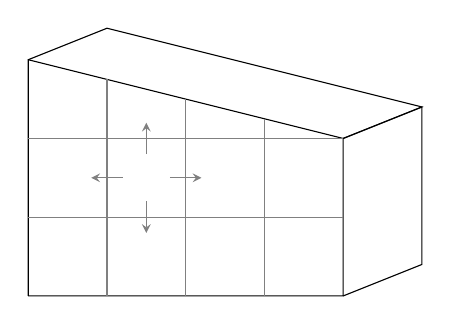
\begin{tikzpicture}
%\draw[gray,step=0.2](0,0) grid (5,4);
%\draw[thick,gray](0,0) grid (5,4);
%volume
\draw (0,0)--(4,0)--(4,2)--(0,3)--(0,0);
\draw (4,0)--(5,0.4)--(5,2.4)--(4,2);
\draw (4,2)--(5,2.4)--(1,3.4)--(0,3);
%squares
\draw[gray] (0,1)--(4,1);
\draw[gray] (0,2)--(4,2);
\draw[gray] (1,0)--(1,2.75);
\draw[gray] (2,0)--(2,2.5);
\draw[gray] (3,0)--(3,2.25);

\draw[gray,-stealth](1.2,1.5)--(0.8,1.5);
\draw[gray,-stealth](1.8,1.5)--(2.2,1.5);
\draw[gray,-stealth](1.5,1.2)--(1.5,0.8);
\draw[gray,-stealth](1.5,1.8)--(1.5,2.2);
%\draw plot[smooth] coordinates {(4,0) (2,0) (1,0.5) (0.4,1) (0,2) (0.5,3) (1.5,3.2) (2.5,3) (2.6,2)  (3,1) (4,0)};
%\shade[rotate=30,shade,ball color=white] ellipse (3 and 2);
\end{tikzpicture}
\end{document}
